\documentclass[12pt,a4paper]{article}

\usepackage[a4paper, top = 2cm, bottom = 2cm, left = 1.5cm, right = 1.5cm]{geometry}
\usepackage[dvipsnames]{xcolor} % Colors

\usepackage{standalone}

\usepackage{setspace}
\usepackage{graphicx}
\usepackage{amsfonts}
\usepackage{amsmath}
\usepackage{tikz}
\usepackage{pdfpages}
\usepackage{epigraph}
\usepackage{csquotes}

% Bibliography
\usepackage{xcolor}
\usepackage{hyperref}
\hypersetup{
    colorlinks=true,
    citecolor=MidnightBlue,
		linkcolor=MidnightBlue,
    pdfpagemode=FullScreen,
    }

\usepackage{natbib}
\usepackage[noabbrev]{cleveref}
\setcitestyle{authoryear,open={(},close={)}}
\bibliographystyle{plainnat}

\usepackage{subfiles}

\setlength\parindent{0pt}
\spacing{1.2}

\begin{document}

\begin{center}
       \vspace*{1cm}
       \huge\textbf{Problemset 2} \\
       \vspace{0.4cm}
       \large \textbf{Public Finance in Macroeconomics} \\
       \vspace{0.5cm}
        \large Handed in by the \textcolor{orange}{\textbf{Heterogeneous Geeks}} \\ 
        \vspace{0.3cm}
        a.k.a. Vivien Voigt, Thong Nguyen, 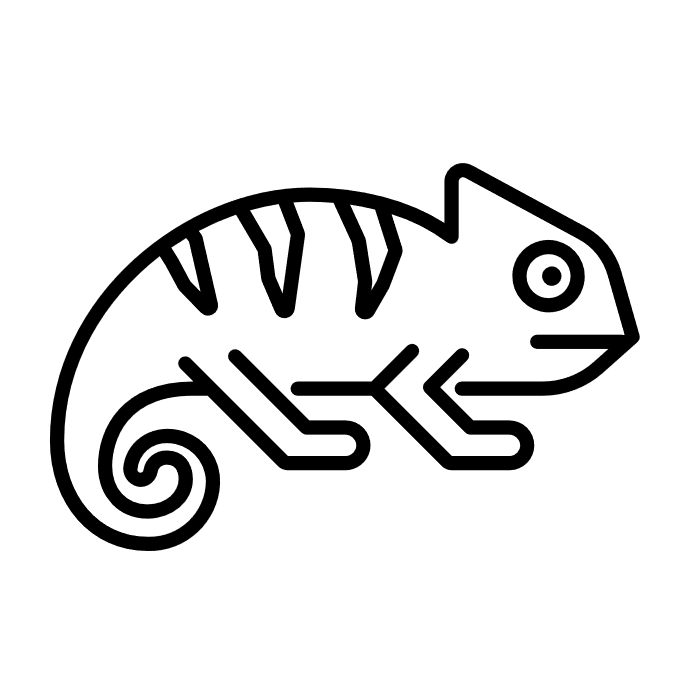
\includegraphics[scale=0.06]{geek.png}\\Davide Difino \& Celina Proffen \\
       \vspace{1.5cm}
       \vfill
       
       % I also thought of adding some cool superheroe image her, but I didn't find one - feel free to delete the gecko if you don't like it/ find it appropriate! ;)
       
        Problem set in the context of Prof. Ludwig's course: \\
        \textbf{Public Finance in Macroeconomics: Heterogenous Agent Models}\\
        at the Graduate School of Economics Finance and Management
       \vspace{0.8cm}
   \end{center}

\newpage
\section*{Problem 1}

Here I first insert all 4 regression tables for quarterly summary statistics.
\begin{table}[htbp]\centering
\def\sym#1{\ifmmode^{#1}\else\(^{#1}\)\fi}
\caption{Summary Quarter 1 \label{sum\_Q1}}
\begin{tabular}{l*{1}{cccccc}}
\hline\hline
            &\multicolumn{1}{c}{(1)}&            &            &            &            &            \\
            &       count&        mean&         var&          sd&         min&         max\\
\hline
hhsize      &       67256&    2.552174&            &    1.517685&           1&          18\\
age         &       67256&    46.93425&            &    17.85164&          14&          94\\
grinc       &       67256&     25143.1&            &    22681.59&      -87243&      423388\\
netinc      &       67256&     22951.4&            &    20433.84&     -150095&      419146\\
food        &       67256&    786.0634&            &    576.6163&           0&       16297\\
ndcons1     &       67256&    2462.707&            &    1726.737&       -3471&       80621\\
ndcons2     &       67256&    1837.486&            &    1238.897&           0&       76066\\
ndconsserv  &       67256&    3200.584&            &    2011.449&        -955&       92337\\
totcons     &       67256&    5264.832&            &    4453.095&          21&       99117\\
\hline\hline
\end{tabular}
\end{table}
\\
\begin{table}[htbp]\centering
\def\sym#1{\ifmmode^{#1}\else\(^{#1}\)\fi}
\caption{Summary Quarter 2 \label{sum\_Q2}}
\begin{tabular}{l*{1}{cccccc}}
\hline\hline
            &\multicolumn{1}{c}{(1)}&            &            &            &            &            \\
            &       count&        mean&         var&          sd&         min&         max\\
\hline
hhsize      &       69977&    2.570959&            &    1.511824&           1&          18\\
age         &       69977&    47.29794&            &    17.67482&          15&          94\\
grinc       &       69977&    25463.11&            &    23011.49&     -103380&      458989\\
netinc      &       69977&    23243.73&            &    20730.42&     -149037&      392936\\
food        &       69977&    788.8158&            &    555.1464&           0&       12553\\
ndcons1     &       69977&    2356.858&            &    1812.279&       -7076&      239060\\
ndcons2     &       69977&    1859.186&            &    1241.181&           0&       72106\\
ndconsserv  &       69977&    3113.207&            &    2130.612&       -2502&      273149\\
totcons     &       69977&    5139.756&            &    4362.793&           6&      209945\\
\hline\hline
\end{tabular}
\end{table}
\\
\begin{table}[htbp]\centering
\def\sym#1{\ifmmode^{#1}\else\(^{#1}\)\fi}
\caption{Summary Quarter 3 \label{sum\_Q3}}
\begin{tabular}{l*{1}{cccccc}}
\hline\hline
            &\multicolumn{1}{c}{(1)}&            &            &            &            &            \\
            &       count&        mean&         var&          sd&         min&         max\\
\hline
hhsize      &       69120&    2.589887&            &     1.52167&           1&          18\\
age         &       69120&    47.56755&            &    17.61981&          15&          94\\
grinc       &       69120&    25521.63&            &    22901.41&      -74324&      493857\\
netinc      &       69120&     23324.9&            &    20708.01&      -96769&      488306\\
food        &       69120&    821.0327&            &    619.2579&           0&       27748\\
ndcons1     &       69120&    2396.207&            &    1688.581&       -1479&       87488\\
ndcons2     &       69120&    1876.569&            &    1307.911&           0&       85746\\
ndconsserv  &       69120&    3181.598&            &    1962.694&           9&      104964\\
totcons     &       69120&    5340.207&            &     4526.06&          10&       95017\\
\hline\hline
\end{tabular}
\end{table}
\\
\begin{table}[htbp]\centering
\def\sym#1{\ifmmode^{#1}\else\(^{#1}\)\fi}
\caption{Summary Quarter 4 \label{sum\_Q4}}
\begin{tabular}{l*{1}{cccccc}}
\hline\hline
            &\multicolumn{1}{c}{(1)}&            &            &            &            &            \\
            &       count&        mean&         var&          sd&         min&         max\\
\hline
hhsize      &       69832&    2.558555&            &    1.525121&           1&          18\\
age         &       69832&    47.16594&            &    17.86099&          16&          94\\
grinc       &       69832&    25074.24&            &    22810.13&      -79767&      490997\\
netinc      &       69832&    22906.24&            &    20568.11&     -151223&      485479\\
food        &       69832&    801.4539&            &    604.5863&           0&       20376\\
ndcons1     &       69832&    2389.181&            &    1719.842&        -587&       81867\\
ndcons2     &       69832&     1838.99&            &    1295.954&           0&       80393\\
ndconsserv  &       69832&    3160.204&            &     2019.21&           0&       94223\\
totcons     &       69832&    5248.625&            &    4517.338&          23&      112698\\
\hline\hline
\end{tabular}
\end{table}
\\

Or, for easily comparing the means in quarterly consumption measures, please see table \ref{compareQs}.

{
\begin{center}
\def\sym#1{\ifmmode^{#1}\else\(^{#1}\)\fi}
\begin{tabular}{l*{1}{cccc}}
\hline
            &\multicolumn{4}{c}{(1)}                            \\
            &\multicolumn{4}{c}{}                               \\
            &    Mean(Q1)&    Mean(Q2)&    Mean(Q3)&    Mean(Q4)\\
\hline
grinc       &  25143.1004&  25463.1111&  25521.6326&  25074.2364\\
netinc      &  22951.4014&  23243.7255&  23324.8959&  22906.2361\\
food        &    786.0634&    788.8158&    821.0327&    801.4539\\
ndcons1     &   2462.7068&   2356.8577&   2396.2071&   2389.1805\\
ndcons2     &   1837.4857&   1859.1858&   1876.5693&   1838.9897\\
ndconsserv  &   3200.5841&   3113.2073&   3181.5983&   3160.2041\\
totcons     &   5264.8319&   5139.7563&   5340.2068&   5248.6255\\
\hline\hline
\end{tabular}
\end{center}
}


\section*{Problem 2}

There are basically two specifications that we want to test. 

\subsection*{Individual Consumption depends only on Aggregate Spending}

This also means, that individual consumption changes co-move one-to-one with the economy's average expenditure changes (and not with individual income changes). We can test this by running the following regression:


Thereby, we can proxy for changes in aggregate spending by \\
a) changes in aggregate income, or
b) changes in aggregate consumption.

In specification b), I will always look at the same type of consumption (i.e. food, non-durables including education, non-durables excluding education, etc.)

Here, I will first only include the regression tables for total consumption (but I have them for all)

a) \ref{totcons\_deltacons} \begin{table}[htbp]\centering
\def\sym#1{\ifmmode^{#1}\else\(^{#1}\)\fi}
\caption{\label{tab:totcons-deltacons} Explaining change in totcons}
\begin{tabular}{l*{2}{c}}
\hline\hline
            &\multicolumn{1}{c}{(1)}         &\multicolumn{1}{c}{(2)}         \\
\hline
agg\_totcons\_shock&       0.991\sym{***}&       0.996\sym{***}\\
            &    (0.0679)         &    (0.0679)         \\
grossinc.change&      0.0255\sym{***}&                     \\
            &   (0.00137)         &                     \\
age         &       3.158\sym{**} &       3.029\sym{*}  \\
            &     (1.192)         &     (1.194)         \\
hhsize      &       47.49\sym{***}&       48.43\sym{***}\\
            &     (13.32)         &     (13.33)         \\
1.quarter   &           0         &           0         \\
            &         (.)         &         (.)         \\
2.quarter   &      -12.65         &      -8.535         \\
            &     (59.45)         &     (59.52)         \\
3.quarter   &      -7.073         &      -7.273         \\
            &     (55.95)         &     (56.02)         \\
4.quarter   &       14.31         &       12.75         \\
            &     (55.19)         &     (55.25)         \\
year        &     -0.0308         &    -0.00331         \\
            &     (0.728)         &     (0.729)         \\
netinc.change&                     &      0.0214\sym{***}\\
            &                     &   (0.00137)         \\
constant    &      -293.7\sym{**} &      -290.9\sym{**} \\
            &     (110.9)         &     (111.0)         \\
\hline
\(N\)       &       44772         &       44772         \\
\hline\hline
\multicolumn{3}{l}{\footnotesize Standard errors in parentheses}\\
\multicolumn{3}{l}{\footnotesize \sym{*} \(p<0.05\), \sym{**} \(p<0.01\), \sym{***} \(p<0.001\)}\\
\end{tabular}
\end{table}


b) \ref{totcons\_deltainc}
\begin{table}[htbp]\centering
\def\sym#1{\ifmmode^{#1}\else\(^{#1}\)\fi}
\caption{\label{totcons\_deltainc} Explaining change in totcons}
\begin{tabular}{l*{2}{c}}
\hline\hline
            &\multicolumn{1}{c}{(1)}         &\multicolumn{1}{c}{(2)}         \\
\hline
agg\_grinc\_~k&  -0.0000445         &                     \\
            & (0.0000831)         &                     \\
diff\_grinc  &      0.0257\sym{***}&                     \\
            &   (0.00138)         &                     \\
age         &       3.387\sym{**} &       3.252\sym{**} \\
            &     (1.195)         &     (1.196)         \\
hhsize      &       46.89\sym{***}&       47.81\sym{***}\\
            &     (13.35)         &     (13.36)         \\
1.quarter   &           0         &           0         \\
            &         (.)         &         (.)         \\
2.quarter   &      -333.3\sym{***}&      -327.4\sym{***}\\
            &     (55.99)         &     (55.87)         \\
3.quarter   &      -105.0         &      -101.5         \\
            &     (55.89)         &     (56.13)         \\
4.quarter   &      -139.7\sym{*}  &      -148.1\sym{**} \\
            &     (56.06)         &     (56.04)         \\
year        &     -0.0830         &     -0.0842         \\
            &     (0.730)         &     (0.731)         \\
agg\_netinc~k&                     &  -0.0000845         \\
            &                     & (0.0000830)         \\
diff\_netinc &                     &      0.0216\sym{***}\\
            &                     &   (0.00138)         \\
constant    &       100.2         &       113.3         \\
            &     (108.8)         &     (109.2)         \\
\hline
\(N\)       &       44772         &       44772         \\
\hline\hline
\multicolumn{3}{l}{\footnotesize Standard errors in parentheses}\\
\multicolumn{3}{l}{\footnotesize \sym{*} \(p<0.05\), \sym{**} \(p<0.01\), \sym{***} \(p<0.001\)}\\
\end{tabular}
\end{table}


\subsection*{Individual Consumption Growth depends only on Aggregate Consumption Growth}

I regress individual HH's consumption growth rates (in its different specifications) in the past 9 months (time between the surveys) on the growth rate of aggregate consumption of that type, the growth rate of the HH's income and HH characteristics such as (age, HH size) and seasonal variation. 

\begin{table}[htbp]\centering
\def\sym#1{\ifmmode^{#1}\else\(^{#1}\)\fi}
\caption{\label{logfood\_deltacons} Explaining change in food}
\begin{tabular}{l*{2}{c}}
\hline\hline
            &\multicolumn{1}{c}{(1)}         &\multicolumn{1}{c}{(2)}         \\
\hline
delta\_logf~g&       0.618\sym{***}&       0.621\sym{***}\\
            &    (0.0489)         &    (0.0490)         \\
delta\_logg~c&      0.0501\sym{***}&                     \\
            &   (0.00385)         &                     \\
age         &    0.000507\sym{***}&    0.000506\sym{***}\\
            &  (0.000152)         &  (0.000152)         \\
hhsize      &     0.00538\sym{**} &     0.00531\sym{**} \\
            &   (0.00169)         &   (0.00169)         \\
1.quarter   &           0         &           0         \\
            &         (.)         &         (.)         \\
2.quarter   &    -0.00990         &     -0.0106         \\
            &   (0.00739)         &   (0.00741)         \\
3.quarter   &     0.00473         &     0.00427         \\
            &   (0.00708)         &   (0.00710)         \\
4.quarter   &     0.00276         &     0.00215         \\
            &   (0.00700)         &   (0.00701)         \\
year        &   -0.000206\sym{*}  &   -0.000208\sym{*}  \\
            & (0.0000930)         & (0.0000931)         \\
delta\_logn~c&                     &      0.0499\sym{***}\\
            &                     &   (0.00391)         \\
constant    &     -0.0279\sym{*}  &     -0.0269         \\
            &    (0.0137)         &    (0.0137)         \\
\hline
\(N\)       &       44573         &       44376         \\
\hline\hline
\multicolumn{3}{l}{\footnotesize Standard errors in parentheses}\\
\multicolumn{3}{l}{\footnotesize \sym{*} \(p<0.05\), \sym{**} \(p<0.01\), \sym{***} \(p<0.001\)}\\
\end{tabular}
\end{table}


\begin{table}[htbp]\centering
\def\sym#1{\ifmmode^{#1}\else\(^{#1}\)\fi}
\caption{\label{tab:logndcons1-deltacons} Explaining change in ndcons1 consumption growth}
\begin{tabular}{l*{2}{c}}
\hline\hline
            &\multicolumn{1}{c}{(1)}         &\multicolumn{1}{c}{(2)}         \\
\hline
log.averagendcons1.change&       0.444\sym{***}&       0.448\sym{***}\\
            &    (0.0399)         &    (0.0400)         \\
lg.grossinc.change&      0.0454\sym{***}&                     \\
            &   (0.00289)         &                     \\
age         &  -0.0000907         &  -0.0000933         \\
            &  (0.000114)         &  (0.000114)         \\
hhsize      &     0.00491\sym{***}&     0.00481\sym{***}\\
            &   (0.00127)         &   (0.00127)         \\
1.quarter   &           0         &           0         \\
            &         (.)         &         (.)         \\
2.quarter   &     -0.0207\sym{***}&     -0.0209\sym{***}\\
            &   (0.00583)         &   (0.00584)         \\
3.quarter   &     -0.0256\sym{***}&     -0.0261\sym{***}\\
            &   (0.00569)         &   (0.00569)         \\
4.quarter   &     -0.0441\sym{***}&     -0.0440\sym{***}\\
            &   (0.00592)         &   (0.00593)         \\
year        &  -0.0000238         &  -0.0000282         \\
            & (0.0000696)         & (0.0000697)         \\
lg.netinc.change&                     &      0.0455\sym{***}\\
            &                     &   (0.00294)         \\
constant    &      0.0318\sym{**} &      0.0326\sym{**} \\
            &    (0.0104)         &    (0.0104)         \\
\hline
\(N\)       &       44641         &       44443         \\
\hline\hline
\multicolumn{3}{l}{\footnotesize Standard errors in parentheses}\\
\multicolumn{3}{l}{\footnotesize \sym{*} \(p<0.05\), \sym{**} \(p<0.01\), \sym{***} \(p<0.001\)}\\
\end{tabular}
\end{table}


\begin{table}[htbp]\centering
\def\sym#1{\ifmmode^{#1}\else\(^{#1}\)\fi}
\caption{\label{tab:logndcons2-deltacons} Explaining change in ndcons2 consumption growth}
\begin{tabular}{l*{2}{c}}
\hline\hline
            &\multicolumn{1}{c}{(1)}         &\multicolumn{1}{c}{(2)}         \\
\hline
log.averagendcons2.change&       0.450\sym{***}&       0.455\sym{***}\\
            &    (0.0438)         &    (0.0438)         \\
lg.grossinc.change&      0.0419\sym{***}&                     \\
            &   (0.00287)         &                     \\
age         &   -0.000396\sym{***}&   -0.000389\sym{***}\\
            &  (0.000113)         &  (0.000113)         \\
hhsize      &     0.00401\sym{**} &     0.00391\sym{**} \\
            &   (0.00126)         &   (0.00127)         \\
1.quarter   &           0         &           0         \\
            &         (.)         &         (.)         \\
2.quarter   &     0.00434         &     0.00397         \\
            &   (0.00524)         &   (0.00525)         \\
3.quarter   &     0.00308         &     0.00245         \\
            &   (0.00531)         &   (0.00531)         \\
4.quarter   &    -0.00962         &    -0.00982         \\
            &   (0.00518)         &   (0.00519)         \\
year        &   0.0000202         &   0.0000181         \\
            & (0.0000692)         & (0.0000692)         \\
lg.netinc.change&                     &      0.0415\sym{***}\\
            &                     &   (0.00292)         \\
constant    &      0.0338\sym{***}&      0.0343\sym{***}\\
            &    (0.0102)         &    (0.0102)         \\
\hline
\(N\)       &       44645         &       44447         \\
\hline\hline
\multicolumn{3}{l}{\footnotesize Standard errors in parentheses}\\
\multicolumn{3}{l}{\footnotesize \sym{*} \(p<0.05\), \sym{**} \(p<0.01\), \sym{***} \(p<0.001\)}\\
\end{tabular}
\end{table}


\begin{table}[htbp]\centering
\def\sym#1{\ifmmode^{#1}\else\(^{#1}\)\fi}
\caption{\label{tab:logndconsserv-deltacons} Explaining change in ndconsserv consumption growth}
\begin{tabular}{l*{2}{c}}
\hline\hline
            &\multicolumn{1}{c}{(1)}         &\multicolumn{1}{c}{(2)}         \\
\hline
log.averagendconsserv.change&       0.413\sym{***}&       0.412\sym{***}\\
            &    (0.0390)         &    (0.0390)         \\
lg.grossinc.change&      0.0317\sym{***}&                     \\
            &   (0.00236)         &                     \\
age         &   0.0000595         &   0.0000537         \\
            & (0.0000931)         & (0.0000932)         \\
hhsize      &    -0.00841\sym{***}&    -0.00854\sym{***}\\
            &   (0.00104)         &   (0.00104)         \\
1.quarter   &           0         &           0         \\
            &         (.)         &         (.)         \\
2.quarter   &     -0.0220\sym{***}&     -0.0221\sym{***}\\
            &   (0.00475)         &   (0.00476)         \\
3.quarter   &     -0.0171\sym{***}&     -0.0175\sym{***}\\
            &   (0.00445)         &   (0.00446)         \\
4.quarter   &     -0.0316\sym{***}&     -0.0318\sym{***}\\
            &   (0.00459)         &   (0.00460)         \\
year        &  -0.0000447         &  -0.0000462         \\
            & (0.0000569)         & (0.0000570)         \\
lg.netinc.change&                     &      0.0299\sym{***}\\
            &                     &   (0.00240)         \\
constant    &      0.0397\sym{***}&      0.0407\sym{***}\\
            &   (0.00850)         &   (0.00851)         \\
\hline
\(N\)       &       44646         &       44448         \\
\hline\hline
\multicolumn{3}{l}{\footnotesize Standard errors in parentheses}\\
\multicolumn{3}{l}{\footnotesize \sym{*} \(p<0.05\), \sym{**} \(p<0.01\), \sym{***} \(p<0.001\)}\\
\end{tabular}
\end{table}


\begin{table}[htbp]\centering
\def\sym#1{\ifmmode^{#1}\else\(^{#1}\)\fi}
\caption{\label{logtotcons\_deltacons} Explaining change in totcons}
\begin{tabular}{l*{2}{c}}
\hline\hline
            &\multicolumn{1}{c}{(1)}         &\multicolumn{1}{c}{(2)}         \\
\hline
delta\_logt~g&       0.390\sym{***}&       0.394\sym{***}\\
            &    (0.0461)         &    (0.0462)         \\
delta\_logg~c&      0.0875\sym{***}&                     \\
            &   (0.00355)         &                     \\
age         &    0.000873\sym{***}&    0.000864\sym{***}\\
            &  (0.000140)         &  (0.000140)         \\
hhsize      &     0.00430\sym{**} &     0.00411\sym{**} \\
            &   (0.00156)         &   (0.00156)         \\
1.quarter   &           0         &           0         \\
            &         (.)         &         (.)         \\
2.quarter   &     -0.0304\sym{***}&     -0.0303\sym{***}\\
            &   (0.00705)         &   (0.00706)         \\
3.quarter   &     -0.0224\sym{***}&     -0.0230\sym{***}\\
            &   (0.00655)         &   (0.00656)         \\
4.quarter   &     -0.0356\sym{***}&     -0.0353\sym{***}\\
            &   (0.00642)         &   (0.00643)         \\
year        &   0.0000783         &   0.0000753         \\
            & (0.0000858)         & (0.0000858)         \\
delta\_logn~c&                     &      0.0857\sym{***}\\
            &                     &   (0.00361)         \\
constant    &    -0.00365         &    -0.00251         \\
            &    (0.0128)         &    (0.0128)         \\
\hline
\(N\)       &       44646         &       44448         \\
\hline\hline
\multicolumn{3}{l}{\footnotesize Standard errors in parentheses}\\
\multicolumn{3}{l}{\footnotesize \sym{*} \(p<0.05\), \sym{**} \(p<0.01\), \sym{***} \(p<0.001\)}\\
\end{tabular}
\end{table}


\end{document}

